% !TEX program = xelatex
\documentclass[12pt]{report}
\usepackage{fontspec}

\defaultfontfeatures{Ligatures=TeX}
% \setmainfont{DidactGothic-Regular}
% \setmainfont{NotoSans-Regular}
\setmainfont{Comfortaa-Regular}

\usepackage[english, bulgarian]{babel}
\usepackage{indentfirst}
\usepackage[a4paper, portrait, margin = 2.0 cm]{geometry}
\usepackage{url}
\usepackage{color}
\usepackage{float}
\usepackage{xcolor}
\usepackage{graphicx}
\usepackage{listings}
\usepackage{subfig}
\usepackage[export]{adjustbox}
\usepackage{blindtext}
\usepackage{scrextend}
\usepackage{amsmath}
\usepackage{amsfonts}

\addtokomafont{labelinglabel}{\sffamily}

\def\changemargin#1#2{\list{}{\rightmargin#2\leftmargin#1}\item[]}
\let\endchangemargin=\endlist 

\renewcommand{\baselinestretch}{1.1}
\setlength{\emergencystretch}{3em}

\usepackage{graphicx}
\graphicspath{ {./resources/} }

\DeclareFontFamily{OT1}{pzc}{}
\DeclareFontShape{OT1}{pzc}{m}{it}{<-> s * [1.5] pzcmi7t}{}
\DeclareMathAlphabet{\mathpzc}{OT1}{pzc}{m}{it}


\lstset{
	backgroundcolor = \color{light-gray},
    language = C,
    xleftmargin = 1cm,
    framexleftmargin = 1em,
    basicstyle=\ttfamily,
	moredelim=[is][\underbar]{_}{_},
}

\usepackage{color}
\definecolor{Bluish}{rgb}{0.39,0.55,0.78}
\definecolor{light-gray}{gray}{0.9}

\usepackage{hyperref}
\hypersetup{
    colorlinks=true,
    linktoc=all,
    citecolor=black,
    filecolor=black,
    linkcolor=black,
    urlcolor=black
}

\usepackage{tabularx}


\title{Дипломна работа}
\author{Диана Генева <dageneva@qtrp.org>}
\date{2018}

\begin{document}
\maketitle
\thispagestyle{empty}
\tableofcontents
\pagebreak

\chapter{Нулева зона}
Бла, бла, бла, аз съм толкова емоционална. 
Не знам

\includegraphics[width=0.5\textwidth ]{pikachu}

\chapter{Емоции в реч}
    \section{Физика на тъгата}
    Вокален тракт е общото название на кухините над ларингса (гръкляна), през които минава въздуха при генериране на реч.
    При хората той се състои от ларингеална кухина, фарингс, устна кухина и носна кухина, които могат да се видят на Фиг. 1.
    Вокалният тракт е отговорен за произвеждане на различни звуци, като текущата конфигурация на отделните му компоненти определя самия звук.
    Според [https://ieeexplore.ieee.org/document/4809202], освен конкретния звук, конфигурацията на вокалния тракт зависи и от емоцията, която изпитва говорещият. 
    Из българската литература се срещат изречения като "страхът стискаше гърлото, задушаваше гласа"[Гласовете ви чувам] и изрази като "буца в гърлото" или "пресъхнало гърло" са станали синоними за дадено емоционално
    състояние в разговорната реч. Тези фрази имат физиологично обяснение и влияят върху характеристиките на произведената реч.
    Именно затова бихме искали да можем математически да моделираме конфигурацията на вокалния тракт и да извличаме характеристики от нея.
    \begin{figure}[ht]%
        \centering
        \begin{changemargin}{0cm}{0cm} 
            \subfloat[Part 1]{%
                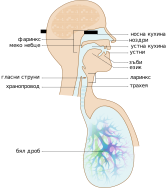
\includegraphics[width=0.48\paperwidth,valign=t]{physics}%
            } \hspace{0.8cm}
            \subfloat[Part 2]{%
                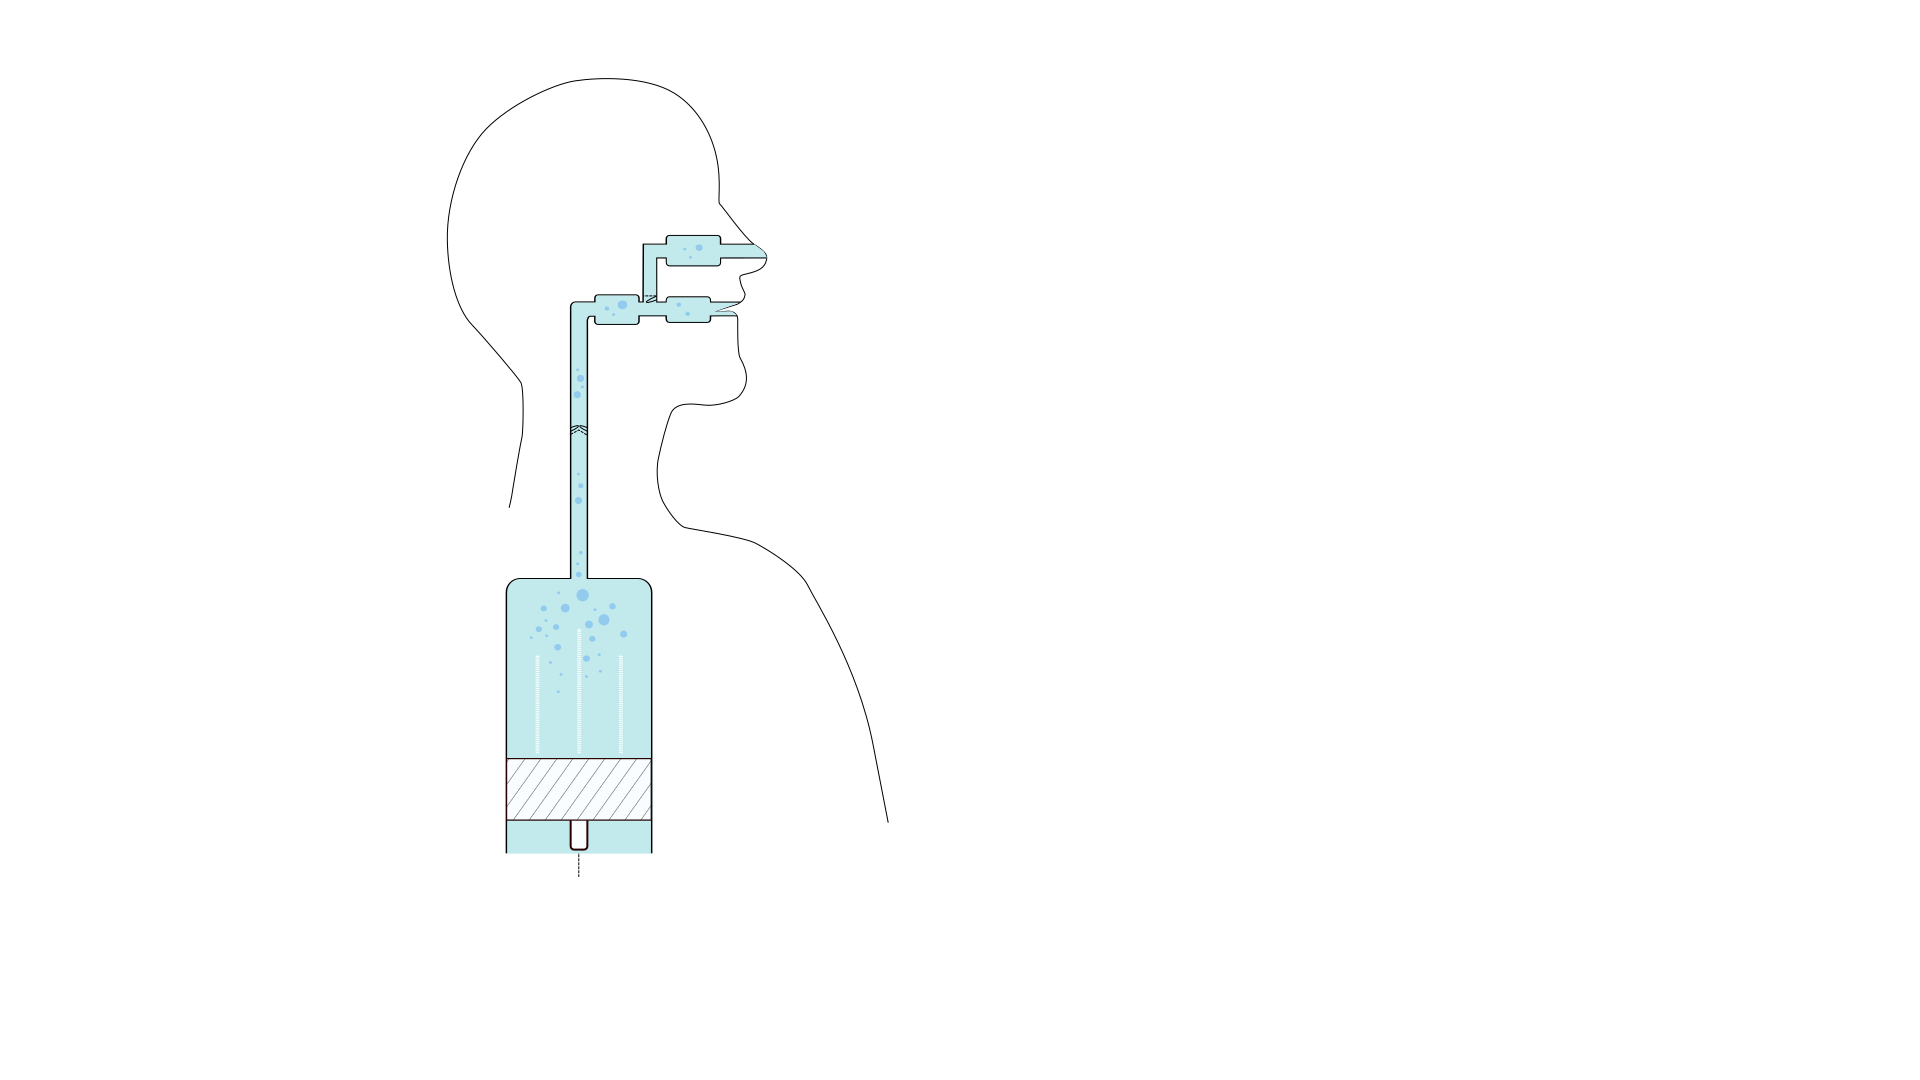
\includegraphics[width=0.28\paperwidth,valign=t]{tubes}%
                \vphantom{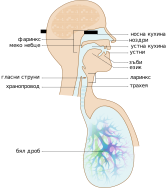
\includegraphics[width=0.48\paperwidth,valign=t]{physics}}%
            }
        \end{changemargin} 

        \caption{Гррррр}%
        \label{fig:example}%
    \end{figure}
    
    Да разгледаме по-подробно Фиг.1 и цялостна система за производство на реч.
    Речта, всъщност, представлява просто акустичната вълна, получена на края на системата - устни и ноздри - в следствие на изкарания от белия дроб въздух.

    Белият дроб работи като енергиен източник за тази системата - въздушният поток, получен при свиването му от междуребрените мускули и диафрагмата,
    се пропагира нагоре по трахеята и през глотиса (отворе между гласните струни). Тъй като налягането в глотиса е по-малко от това в който и да е от двата му края, по закона на Бернули
    в някакъв момент става толкова ниско, че позволява на гласните струни да се затворят. В следствие се натрупва налягане зад гласните струни, което в някакъв момент ги принуждава
    да се отворят и цикълът се повтаря отначало. В резултат се получава осцилиране на гласните струни. Честотата на отварянето и затварянето зависи от анатомични особености като еластичността и големината на
    гласните струни, налягането в белия дроб и други. При мъжете тази честота е средно 125 Hz, а при жените - 210 Hz. Акустичната вълна, която се получава в следствие на осцилацията,
    преминава през вокалния тракт, където се завихря, при срещане на прегради, като устни и зъби, и в крайна сметка напуска системата през някой от отворите.

    При целият този процес се губи част от енергията, поради различни фактори: стените на вокалния тракт са меки и еластични, радиацията на вълната при устните и ноздрите и други.

    В зависимост от начинът, по който вълната напуска системата, можем да класифицираме произведените звуци по следния начин:

    \begin{enumerate}
        \item Озвучени 
        При тези звуци гласните струни осцилират квази-периодично.
        \item Проходни (фрикативни) 
        При образуването на проходни звуци, вълната среща преграда по пътя си
            (като например зъби, устни), и се получава турболенция при опита въздухът да бъде избутан през преградата
        \item Преградни (експлозивни)
        Те се получават, когато преградата е пълна, което позволява да се натрупа налягане
        зад съответната прегада, което се освобождава рязко.
    \end{enumerate}
    
    Ако разгледаме вокалния тракт и носната кухина като свързани тръби с непостоянно напречно сечение и вземем предвид горното описание за генериране на звук,
    то честотният спектър ще зависи от честнотната пропускливост на тръбите (frequency selectivity) Трябва да видя онова в тетрадката. Това много прилича на свирене на духов инструмент.
    Честотите на които се получава резонанс зависи от формата и размера на тръбите. Известно е, че за да се образува определен звук, трябва да се промени формата на вокалния тракт по 
    съответния начин. (Например, когато човек казва "н" езикът се залепя зад зъбите и т.н.). В такъв случай, спектралните особености на сигнала се менят с времето, тъй като се мени и
    положението на вокалния тракт. Смята се [], че състоянието на вокалния тракт е сравнително статично (достатъчно статично за нашите цели) в рамките на 15ms, преди да се смени съответната
    фонема, която се изговаря. В такъв случай, можем да излседваме спектралните свойства в този отрязък от време и да извличаме информацията за подлежата емоция в него. 

    \section{Загладено опростяване}
    За улеснение, нека разгледаме конкретна конфигурация, за да се опитаме да я моделираме математически. Например тази, при произнасянето на фонемата "ъ", тъй като е възможно най-проста.
    
    В случая на гласната "ъ", глотиса трепти, а клапата към носната кухина е затворена и само устната кухина участва в образуването на звука. 
    Т.е. имаме някакъв източник на псевдо-периодично трептене $\mathpzc{U}$ - глотис, после вълната преминава и се променя от вокалния тракт $\mathpzc{V}$ и накрая излиза и се пречупва през
    устните $\mathpzc{R}$. Сигналът, който получаваме накрая е $\mathpzc{Y}(z) = \mathpzc{U}(z)\mathpzc{V}(z)\mathpzc{R}(z)$
    и това, от което се интересуваме е $\mathpzc{V}$.
    \begin{figure}[ht]%
        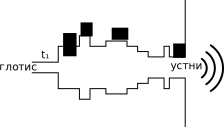
\includegraphics[width=\textwidth]{vocal_tubes}%
        \caption{Приближение на вокалния тракт с $k$ тръби}%
    \end{figure}
    Нека устната кухина е приближена с $k$ на брой тръби с постоянно напречно сечение, както е показано на Фиг.2.
    За още по-голямо опростяване нека няма и загуба на енергия, каквата би се получила попринцип.

    Нека въведем следните стандартни означения:
    \begin{enumerate}
        \item{$\mathpzc{c}$} - скорост на звука , т.е. това е разстоянието, което пропътува вълната за единица време
        \item{$\rho$} - плътност на въздуха
        \item{$\mathcal{A}$} - напречно сечение
        \item{$u$} - обемна скорост
        \item{$p$} -  налягане - можем да си мислим за него като "колко сила е нужна, за да се преместят частитиците"
    \end{enumerate}
    
    Тъй като въздухът е течна среда, как пътува вълна през него се определя от свойствата на въздуха и от ограниченията на тръбата като дължина и ширина. Звуковите вълни, преминаващи през
    тръба изпълняват уравнения [Rabiner and Schafer, pg 59, (3.2a) (3.2b)]:
    
    \begin{equation}
       -\frac{\partial\rho}{\partial x} = \frac{\rho}{\mathcal{A}} \frac{\partial u}{\partial t}
        \label{eq:litdiff}
    \end{equation}
        
    \begin{equation}
        -\frac{\partial u}{\partial x} = \frac{\mathcal{A}}{\rho \mathpzc{c}^2} \frac{\partial \rho}{\partial t}
         \label{eq:litdiff}
     \end{equation}
    
    при преминава от една тръба в друга, част от вълните ще преминат към следващата тръба, а част от тях ще се отразят в наобратно. В такъв случай във всеки момент от време
    $t$ и във всяка точка $x$ на всяка тръба обемната скорост $u$ ще зависи от обемната скорост на вълните, които вървят "напред" и тази на вълните, които вървят "назад". Затова може да се покаже,
    че уравненията (2) имат решение във следния вид:

    \begin{equation}
        u_{k}(x, t) = [u_{k}^{+}(t - \frac{x}{\mathpzc{c}}) - u_{k}^{-}(t + \frac{x}{\mathpzc{c}})]
        \label{eq:litdiff}
    \end{equation}

    \begin{equation}
        p_{k}(x, t) = \frac{\rho \mathpzc{c}}{\mathcal{A_{k}}} [u_{k}^{+}(t - \frac{x}{\mathpzc{c}}) + u_{k}^{-}(t + \frac{x}{\mathpzc{c}})]
        \label{eq:litdiff}
    \end{equation}

    където 
    \begin{enumerate}
        \item{$t_{k}$} е $k$-тата тръба, която има дължина $l_k$ и лице на напречното сечение $A_k$
        \item{$x$} е разстояние в $t_k$ ($0\leq x \leq l_k$)
        \item{$t$} е момент от време
        \item{$u^{+}$ и $u^{-}$} са съответно вълните, които вървят "напред" и тези, които вървят "назад"
    \end{enumerate}

    \section{Характеристики}
        \subsection{Избор}
        \subsection{Извличане}

        Първо се изчита wav файла, като данни се запазват в масив от float числа. Базирайки се на идеята, че
        че вокалния тракт е статичен за много къс период от време, накъсваме масива с данните на
        отделни застъпващи се фреймове, в рамките на които сигналът е статичен ("представяме си, че е статичен"). За да получим добра
        добра честотна резолюция, трябва да се включат голям брой samples от файла, но колкото по-голяма е дължината
        на фрейма, толкова по-голям е шансът да включим данни за различни конфигурации на глотиса.
        За да се постигне някакъв trade-off между двете, обикновено стойностите, които се избират, са 
        25 милисекунди за дължина на фрейм и 10 милисекунди за разстояние между два последователни фрейма.[Paul]
        
        Тъй като алгоритъмът за извличане на mfcc коефициенти, изисква броя на самплите да е степен на 2,
        допълваме последните фреймове с 0, ако това е нужно, тъй като това не влияе на точността. [мжое би онази статия за fourier]

        




    \section{Класификация}    
    \section{Резултати}

\chapter{Грубо в мозъка}
    \section{Характеристики}
        \subsection{Избор}
        \subsection{Извличане}
    \section{Класификация}    
    \section{Резултати}
\chapter{Двойната звезда}
    \section{Резултати}
\chapter{Големият портрет}


\end{document}